%IMPORTS
\documentclass[a4paper, 11pt]{article}
\usepackage[utf8]{inputenc} 
\usepackage[T1]{fontenc}
\usepackage[catalan]{babel}
\usepackage{amsmath, amssymb, amsthm}
\usepackage[margin=1in]{geometry}
\usepackage{enumerate}
\usepackage{array}
\usepackage{graphicx}
\usepackage{wrapfig}
\usepackage{ragged2e} 
\usepackage{subfig}
\usepackage{caption}
\usepackage{subcaption}
\usepackage[dvipsnames]{xcolor}
%\usepackage[table]{xcolor}
\usepackage{float}
\usepackage{chngcntr}
\usepackage{ragged2e}
\usepackage{multirow}
\usepackage{vmargin}
\usepackage{hyperref}
\usepackage{url}
\usepackage{fancyhdr}
\usepackage{bigints}
\usepackage{listings}
\usepackage{xcolor,colortbl}
\usepackage{arydshln}
%\usepackage{slashbox}


\definecolor{navy}{rgb}{0,0,128}
\definecolor{codegreen}{rgb}{0,0.6,0}
\definecolor{codegray}{rgb}{0.5,0.5,0.5}
\definecolor{codepurple}{rgb}{0.58,0,0.82}
\definecolor{backcolour}{rgb}{0.95,0.95,0.92}
\definecolor{amaranth}{rgb}{0.9, 0.17, 0.31}
\definecolor{GRAY}{rgb}{0.75, 0.75, 0.75}
\definecolor{deepfuchsia}{rgb}{0.76, 0.33, 0.76}
\definecolor{deepmagenta}{rgb}{0.8, 0.0, 0.8}
\definecolor{funcblue}{rgb}{0.36, 0.57, 0.9}

\lstdefinestyle{mystyle}{
    backgroundcolor=\color{white},   
    commentstyle=\color{codegreen},
    keywordstyle=\color{RoyalBlue},
    numberstyle=\tiny\color{codegray},
    stringstyle=\color{codepurple},
    basicstyle=\ttfamily\footnotesize,
    breakatwhitespace=false,         
    breaklines=true,                 
    captionpos=b,                    
    keepspaces=true,                 
    %numbers=left,                    
    numbersep=5pt,                  
    showspaces=false,                
    showstringspaces=false,
    showtabs=false,                  
    tabsize=2
}
\lstdefinestyle{Bash}
{language=bash,
keywordstyle=\color{blue},
basicstyle=\ttfamily,
morekeywords={peter@kbpet},
morekeywords=[2]{make},
keywordstyle=[2]{\color{blue}},
literate={\$}{{\textcolor{blue}{\$}}}1 
         {:}{{\textcolor{blue}{:}}}1
         {~}{{\textcolor{blue}{\textasciitilde}}}1,
}
\lstdefinestyle{BASH}
{language=bash,
keywordstyle=\color{blue},
basicstyle=\ttfamily,
morekeywords={peter@kbpet},
morekeywords=[2]{make},
fontsize=5pt
keywordstyle=[2]{\color{blue}},
literate={\$}{{\textcolor{blue}{\$}}}1 
         {:}{{\textcolor{blue}{:}}}1
         {~}{{\textcolor{blue}{\textasciitilde}}}1,
}

\lstset{style=mystyle}

\setpapersize{A4}
\setmargins{2.5cm}     % margen izquierdo
{2.6cm}                % margen superior
{16.5cm}               % anchura del texto
{23.7cm}               % altura del texto
{10pt}                 % altura de los encabezados
{0cm}                  % espacio entre el texto y los encabezados
{0pt}                  % altura del pie de página
{1cm}                  % espacio entre el texto y el pie de página
\renewcommand{\baselinestretch}{1.5}
\begin{document}

\begin{titlepage}
    \centering
    {\bfseries\LARGE \hspace{1.9em} Universitat Autònoma de Barcelona\newline Facultat de Ciències\par}
    \vspace{2cm}
    {\hspace{-1em}
\includegraphics[width=0.4\textwidth]{logo.png}\par}
    \vspace{1cm}
    {\scshape\Huge Informe Pràctic Etiquetador\par} 
    \vspace{1cm}
    {\Large \itshape Autors: \par}
    {\Large \hspace{0.7em}Gerard Lahuerta \& Ona Sánchez \& Manuel Arnau \& Andrea González\par}
    {\Large 1601350 --- 1601181 --- 1597487 --- 1603921\par}
    
    \vspace{1cm}
    {\Large 29 de Maig del 2022\par}
\end{titlepage}

\justifying

\newpage
\setcounter{page}{2}
\pagestyle{plain}
\tableofcontents
\cleardoublepage
\addcontentsline{}{chapter}{}
\newpage

\section{Introducció i plantejament}
En aquest apartat s'explicarà tot el plantejament que s'ha dut a terme a l'hora d'implementar les millores al classificador, els convenis escollits per a la resolució de problemes que han aparegut, l'explicació d'aquests problemes, els nostres objectius i com s'han triat certs paràmetres per a l'estudi dels resultats.
\subsection{Metodologia i filosofia del treball}
Primerament explicar els nostres objectiu per al classificador:
\begin{enumerate}
    \item Programar un classificador suficientment versàtil com per que s'adapti a diverses situacions de treball (que el programa pugui treballar de diverses maneres).
    \item Fer que el programa pugui variar entre diverses formes de classificar mitjançant especificacions (que trobi els millors paràmetres per a la classificar les dades introduïdes).
    \item Que el canvi de mètode de funcionament del classificador sigui fàcil de fer i de manera intuitiva (que l'usuari pugui especificar quin mode de funcionament vol utilitzar en cada moment).
    \item Optimitzar al màxim el funcionamnt intern del programa mitjançant llibreries especialitzades per l'anàlisis de dades així com per a l'estudi de les mateixes (\textcolor{LimeGreen}{numpy},  \textcolor{LimeGreen}{mathplotlib}, \textcolor{LimeGreen}{seaborn}, \textcolor{LimeGreen}{collections}, \textcolor{LimeGreen}{pandas}, \textcolor{LimeGreen}{multiprocessing}, ...).
    \item Augmentar la precisió del classificador mitjançant mètodes alternatius per l'anàlisi de les dades.
    \item Augmentar l'eficiència (disminuir el cost de temps de computació) del programa mitjançant algoritmes diversos.
    \item Afegir un conjunt de funcions que permetin analitzar de manera més natural i intuitiva els resultats del classificador.
    \item Afegir un conjunt de fucions que permetin observar el rendiment (en temps i en precisió) dels resultats obtinguts pel classificador.
    \item Plantejar mètodes, algoritmes o formes que millorin el classificador (no ens enfoquem en trobar la seva versió més òptima, només si milloren o no).
    \item Distribuir la càrrega de treball entre processos d'execució.
\end{enumerate}
\newpage

\subsubsection{Problemes a l'hora del desenvolupament del procés}
Durant el plantejament de les funcions a implementar i decidir els nostres objectius van sorgir un seguit de problemes que haviem de solucionar/posar el grup d'acord en com treballar amb ells. Aquests problemes/qüestions varen ser:
\begin{enumerate}
    \item Com considerem si el classificador de colors aproxima correctament els colors (ja que la percepció dels mateixos és una experiencia subjectiuva).
    \item Prioritzar la precisió dels classificadors respecte a l'eficiència, o viceversa.
    \item A partir de quin valor podem afirmar que el nostre classificador ha obtingut un conjunt de clústers per classificar suficients.
    \item Quins colors són rellevants en una imatge.
    \item A partir de quin percentatge de precisió considerem que el classificador funciona correctament.
    \item Com ha d'actuar el classificador quan hi pot haver un conflicte en els resultats o hi pot existir un "dubte"\hspace{0.0625em} al hora d'etiquetar.
    \item Com calculem la precisió dels resultats.
    \item Quanta informació es necessària per a classificar i a partir de quan es informació redundant o rellevant.
    \item Quans veins fa falta observar per a obtenir un resultat precís.
    \item Els mètodes son realment eficients de forma general o es tracta d'un fenòmen particular.
    \item Com decidim si un mètode és eficient.
    \item Com asegurem la precisió dels resultats obtinguts en cas de no disposar del \textit{ground truth}.
    \item Quan és necesari aplicar mètodes per distribuir la càrrega de treball de manera òptima.
\end{enumerate}
Per tal de donar solució i poder treballar amb aquestes qüestions s'ha arribat als convenis explicats en el següent apartat.

\newpage

\subsubsection{Convenis i decisions}
Expliquem ara les decisions preses i els convenis escollits per a solucionar les qüestions explicades a l'apartat anterior:
\begin{enumerate}
    \item S'introdueixen cinc criteris de càlcul de percentatges per calcular la precisió dels resultats. Escollim dentre tots aquests percentatges l'explicat a l'apartat \textcolor{blue}{\ref{matriucolors}}.
    \item S'ha decidit prioritzar la precissió davant l'eficiència del temps d'execució. Tot i així es treballarà per a fer els processos eficients en temps.
    \item S'estudiarà el conjunt d'imatges de la nostra base de dades i es plantejaran mètodes per eliminar colors innecessaris (colors de fons, colors residuals...). S'explica a l'apartat \textcolor{blue}{\ref{depuratge}}.
    \item S'acceptarà un funcionament correcte del classificador quan aquest obtingui una precisió superior o igual al $95\%$. 
    \item En cas de que el classificador tingui "dubtes"\hspace{0.0675} al hora d'etiquetar procedirà a etiquetar la mostra de dues maneres. Preferim mostrar informació de més que no pertany al conjunt correcte que no mostrar dades del conjunt. S'explica a l'apartat \textcolor{blue}{\ref{dosetiquetes}}.
    \item Calculem la precisió dels resultats obtinguts a partir d'una subsecció de les dades (que anomenem \textit{data\_test}) que si disposem de les seves etiquetes correctes. Tot i així hi ha processos que per el seus sistema/algorisme ens impedeix utilitzar aquest recurs; s'usa a l'apartat \textcolor{blue}{\ref{crossvalidation}}.
    \item Es dedueix de maner intutitiva que no tota la informació és rellevant, pel que comprovem si l'hipòtesis es correcta comparant la precisió obtinguda agafant informació aleatòria i tot el conjunt d'informació.
    \item Es programarà una funció que estudiarà el nombre òptim de veins a observar per tal d'obtenir la precisió màxima. S'estudia aquest valor als apartats \textcolor{blue}{\ref{crossvalidation}} i \textcolor{blue}{\ref{bestkstatistics}}.
    \item Per cada comprovació dels resultats obtinguts i per tal de fer una anàlisis de forma adecuada és repetiran varies vegades la classificació per tal d'obtenir un resultat suficientment precís com per a afirmar si es tracta o no d'un mètode precís de forma general.
    \item Definim un mètode eficient com aquell que és ràpit executant els càlculs i no obté una precisió inferior al $40\%$. Per tant, decidim si un mètode és eficient o no si segueix aquest criteri i comparem eficiències mitjançant la proporció $\frac{accuracy}{temps}$.
    \item En casos on no es disposa d'una precissió suficientment bona es decidirà (degut a la falta d'un \textit{ground truth}) fer un interval de confiança dels resultats obtinguts; com és el cas de l'apartat \textcolor{blue}{\ref{crossvalidation}}.
    \item Considerarem que és necesari aplicar mètodes d'execució paral·lela (multiprocessing) si obtenim un treball de computació tan elevat que a priori (amb la primera execució) no obtenim els resultats abans d'haber pasat 5 minuts de l'inici de l'execució (considerant que és probable que hi existeixi una diferència de $\pm3$ minuts entre executar el programa en ordinadors amb diveres especificacions i capacitats).
\end{enumerate}
\newpage

\subsection{Plantejament dels anàlisis}
S'ha decidit plantejar l'anàlisis mitjançant representacions gràfiques dels resultats obtinguts per tal d'observar les conclusions de forma més visual. \\
També s'ha decidit implementar millores alternatives al classificador per a comparar l'eficiència i la precisió dels resultats amb el model default.\\
Aquestes millores s'expliquen a continuació, classificades en implementades i no implementades amb l'argumentació del perquè.
\subsubsection{Millores implementades}\label{millores_implementades}
Enunciem ara les millores implementades amb el seu funcionament i referencies a l'explicació detallada de cadascuna d'elles.\\
\underline{Inicialització dels centroides del Kmeans}
\begin{itemize}
    \item Mitjançant una llista de colors preestablerta (concretament amb els 11 colors bàsics que hi disposem a les imatges). Inicialitzar els primers K-clusters escollint de manera aleatòria (sense reposisió) de la llista mencionada. 
    \item Escollir aleatòriament un punt RGB de la imatge i calcular els següents (k-1)-clusters de manera que les distàncies entre ells siguin màximes.
\end{itemize}
\underline{Heurístiques per a la tria de millor nombre de clústers}
\begin{itemize}
    \item Agafar aleatòriament un $x\%$ de la imatge. Classificar els píxels en colors i aquest serà el valor inicial de clústers (es tracta d'una implementació que limita inferiorment el nombre de clústers). 
    \item Agafar 1 de cada 200 píxels de la imatge recorrent els píxels d'esquerra a dreta i de dalt a baix. Classificar els píxels en colors i aquest serà el valor inicial de clústers (es tracta d'una implementació que limita inferiorment el nombre de clústers).
    \item Implementar diferents heurístiques per decidir el valor òptim de K. S'implementaran les heurístiques de $ICD$ i $FD$ (\textit{Inter Class Distance} i \textit{Fisher Distance} respectivament). 
    \item Trobar la millor relació entre valors de distancia obtinguda per tal d'evitar fer càlculs de més i/o obtenir un nombre de clústers superior dels necessaris. 
\end{itemize}
\newpage
\hspace{-1.5em}\underline{Mètodes de depuratge de la imatge}\label{depuratge}
\begin{itemize}
    \item Crear una funció encarregada de depurar el color, irrellevant, del fons de l'imatge.
    \item Crear una funció encarregada de depurar el color, irrellevant, del model que du la roba posada.
\end{itemize}
\underline{Obtenir el valor òptim de veïns a consultar}
\begin{itemize}
    \item Calcular el valor òptim de veïns a consultar a l'hora d'etiquetar avaluant l'accuracy obtinguda per a diversos valors. S'han implementat els mètodes \textcolor{funcblue}{CrossValidation} i \textcolor{funcblue}{best\_k\_statistics()} que recullen aquests objectiu.
\end{itemize}
\underline{Obtenir una millor precisió per la forma}\label{dosetiquetes}
\begin{itemize}
    \item Calcular l'àrea de les imatges (proporció fons-figura) i comparar proporcions.
    \item Aplicar una transformació de color (passar de $RGB$ a escala de grisos) a les imatges per a comparar-les amb menys informació no decisiva i fixar-nos més en les propietats de les formes (no pas els seus colors). 
    \item Atribuir dues etiquetes a una imatge en cas de que l'etiqueta més repetida d'entre els veïns observats no superi un llindar.
\end{itemize}
\newpage

\subsubsection{Millores descartades}
A l'hora d'implementar les millores proposades a l'esborrany, algunes van ser descartades al prioritzar la relació temps dedicat / resultats. En aquest apartat es presentaran aquestes propostes que no es van dur a la pràctica:\\
\underline{Heurístiques per trobar la millor K al kmeans}
\begin{itemize}
    \item Escollir píxels d'una imatge segons dues distribucions normals, una per l'eix $x$ i una per l'eix $y$, amb paràmetres ($\mu$,$\sigma^2$) a escollir experimentalment. Un cop escollits els píxels, usaria la funció \textbf{\textcolor{funcblue}{get\_colors()}} de l'arxiu \textcolor{LimeGreen}{utils} per classificar els color trobats, i inicialitzar la $k$ amb el nombre de colors trobats.\\
    Aquesta idea va ser descartada ja que es van trobar idees més senzilles que disminuien el temps de còmput per trobar la millor $k$, explicades anteriorment a l'apartat \textcolor{blue}{\ref{millores_implementades}}.
    \item Usar la Dimensió de Minkowski. Consisteix en utilitzar la següent fòrmula de la dimensió fraccionaria de Minkowski per mesurar lo bo que és el clúster. 
    \begin{center}
        $dim_{caja}(S) = n - \lim_{r \to 0} \frac{log \hspace{0.3em}vol(S_r)}{log\hspace{0.3em} r}$ 
    \end{center}
    El que es fa és dividir l'espai (cub inicial) en 4 subcubs. Mesurem què tan bo és el clúster a partir del volum de cubs que ocupa i la idea principal consisteix en relacionar en quants cubs s'ha hagut de dividir l’espai per tal que en un cub no aparegui més d’un clúster (iterant fins que això passi). Faltaria veure la relació entre les iteracions de reducció i el volum.\\
    La idea va ser descartada degut a la falta de temps per dur a terme la implentació juntament amb l'alt cost computacional que comportaria.
\end{itemize}
\underline{Trobar la millor K al KNN}\\
Els mètodes que van ser proposats consistien en diverses maneres de determinar el nombre de clústers en un conjunt de dades.
\begin{itemize}
    \item Aplicar el \textit{Silhouette method}. Aquest mètode calcula els coeficients de la \textit{silhouette} de cada punt, que mesuren que tant semblant és un punt amb el seu propi clúster en comparació amb altres clústers. El valor de la silueta va de $-1$ a $1$, on un valor alt indica que el punt està ben aparellat amb el seu clúster.
    \item Combinació de \textit{Silhouette method} amb \textit{l'Elbow Method}. Consisteix en representar la variació de la \textit{silhouette} en funció del nombre de clústers, i escollir l’\textit{elbow} de la corba com el nombre de clústers a utilitzar.
 
\end{itemize}
\underline{Mètodes pel KNN}\\
\begin{itemize}
    \item Canvi de l'espai. Consisteix en canviar l'espai de tractament de les dades, per exemple, passant-lo a coordenades polars per reduir la dimensió guardant tanta informació com sigui possible.
    \item Comparació de les imatges amb uns quants models escollits de forma aleatòria de cada classe. S’etiquetaria a partir de quin és el més semblant. Es repetiria aquest procés K vegades (cal escollir la K més eficient prèviament) per anar comparant amb diferents models. Es dona també una segona opció, fer-ho només un cop, amb un model de cada etiqueta (que podria ser escollit de forma aleatòria o no). Aquest mètode seria el més ràpid, però requeriria un anàlisi la seva precisió, per aquest motiu, es va descartar la proposta.
    \item Usar el CrossValidation per veure en quines peces de roba hi pot haver més dubtes a l'hora de ser etiquetades. Consisteix en entrenar a la vegada diferents mostres del \textit{train dataset}, fer un \textit{predict} amb cadascun, i escollir la forma de roba més repetida. Degut a que aquest mètode no afectaria en la millora de la \textit{accuracy} i l'aplicació de tècniques més senzilles per l'etiquetatge de la roba explicades anteriorment (donar dues etiquetes enlloc d'una en cas de dubte), aquest mètode va ser rebutjat. Tot i així s'usa el Cross Validation per trobar el millor valor de la K en l'algorisme del KNN, l'explicació es troba a l'apartat \textcolor{blue}{\ref{crossvalidation}}.
\end{itemize}
\underline{Altres}
\begin{itemize}
    \item Implementació de \textit{Multiprocessing} a tot el programa. Es va decidir implementar el \textit{multiprocessing} per realitzar l'estudi de la millor $K$ a utilitar pel \textit{KNN} mitjançant un \textit{Cross Validation}. Degut al baix cost computacional de la resta de càlculs del programa, es va decidir que no era necessari implementar aquesta millora a la resta de funcions de l'etiquetador, tot i que si es treballés amb un \textit{dataset} més gran, seria una opció a tenir en compte.
    \item Analitzar la variànça de les matrius que conformen cada imatge, i un cop calculada, comparar amb les variànces amb les matrius de les imatges a etiquetar, de manera que per decidir com etiquetar una imatge, el que es farà es comparar la variànça d'aquesta. Degut a la dificultat del mètode i el poc temps per dur-lo a terme, es va decidir rebutjar la proposta. 
\end{itemize}
\newpage

\section{Anàlisi qualitatiu}
Per veure el funcionament del KMeans i KNN programats per a obtenir uns resultats preliminars i a partir d'aquests veure quines millores serien necessàries implementar, es va començar fent un anàlisi qualitatiu. Aquest anàlisi es duria a terme a partir de les etiquetes que proporcionaven el KMeans i el KNN ja implementats (en els apartats anteriors de la pràctica), mitjançant funcions que retornessin per pantalla aquelles imatges que tinguessin les etiquetes especificades en \textit{"queries"}.\\ Les funcions implementades en aquesta part de l'anàlisi han estat: \textbf{\textcolor{funcblue}{retrieval\_by\_color()}}, \textbf{\textcolor{funcblue}{retrieval\_by\_shape()}} i \textbf{\textcolor{funcblue}{retrieval\_combined()}}, que s'expliquen als apartats \textcolor{blue}{\ref{colors}}, \textcolor{blue}{\ref{shape}} i \textcolor{blue}{\ref{combined}} respectivament.


\newpage

\subsection{Retrieval\_by\_color}\label{colors}
\subsubsection{Cdoc}
\begin{itemize}
    \item Entrada: 
    \begin{itemize}
        \item[$\circ$] Llista d'etiquetes de colors: \textbf{\textcolor{Turquoise}{kmeans\_colors}}
        \item[$\circ$] Llista amb la proporció de cada color a la imatge: \textbf{\textcolor{Turquoise}{proportions\_colors}}
        \item[$\circ$] Imatges etiquetades: \textbf{\textcolor{Turquoise}{imag}}
        \item[$\circ$] Llista de string que conté els colors que es volen filtrar: \textbf{\textcolor{Turquoise}{question}}
    \end{itemize}
    \item Sortida: Conjunt d'imatges que contenen els colors desitjats.
    \item Funcionament: \\
    Per a cada imatge es comprova si té els colors desitjats, i en cas afirmatiu es guarda l'índex de la imatge i també el percentatge que representa el color o els colors dins la imatge. Un cop comprovades totes les imatges, la llista d'índexs és ordenada en ordre descendent segons el percentatge que té cada imatge, i llavors es mostren aquestes ordenades mitjançant la funció \textcolor{funcblue}{visualize\_retrieval()} de la llibreria \textcolor{LimeGreen}{utils}.
\end{itemize}
Els primers resultats obtinguts van permetre veure que hi havia problemes amb un excés en els colors etiquetats, ja que tot i que tinguèssin un percentatge irrellevant eran afegits, amb el fons de les imatges (principalment el blanc) i amb les persones, que eran identificades com a taronges.
\begin{figure}[h!]
\centering
\begin{minipage}{.5\textwidth}
  \centering
  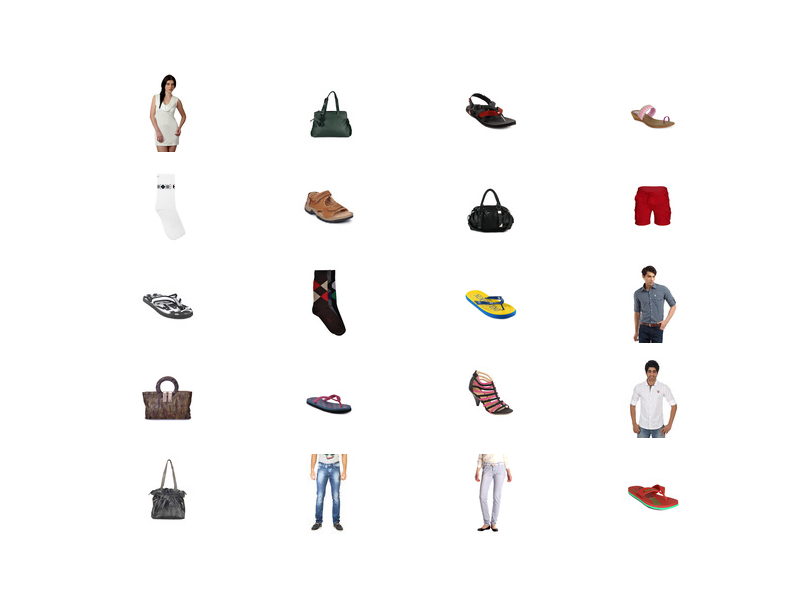
\includegraphics[width=.6\linewidth]{blancosmalos.png}
  \caption*{50 primers White}
\end{minipage}%
\begin{minipage}{.5\textwidth}
  \centering
  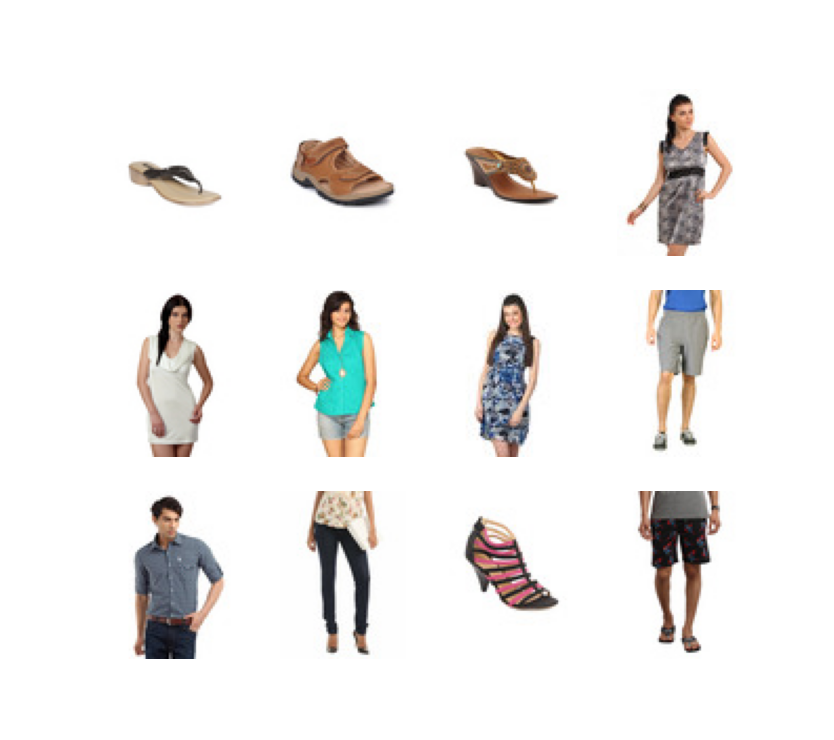
\includegraphics[width=.5\linewidth]{naranjito_malo.png}
  \caption*{50 primers Orange}
\end{minipage}
\end{figure}
\label{millores_filtratge_colors}\\Això va portar a implementar les millores següents ja mencionades als primers apartats: l'eliminació en la major mesura possible del background, mirant les cantonades de la imatge per a saber de quin color és el background i passar la imatge a grisos per facilitar l'eliminació d'aquest, treure la persona (en cas que aparegui) i finalment seleccionar només els colors rellevants de la imatge.\\
La funció de background s'utilitza només al inici del Kmeans, per tal de no generar problemes depenent de com s'inicialitzi. Primer de tot es passa a gris amb la funció \textcolor{funcblue}{rgb2gray()} i després es busca de quin color és el background buscant els extrems, i escollint el color més comú que  aparegui (també es va sopesar la possibilitat d'estudiar tot el contorn, però resultava més costós computacionalment i aquest mètode ja funcionava correctament). Un cop es té el color del background, s'eliminen tots els colors que estan dins l'interval $\{col. background -14, \hspace{0.1em}col. brackground + 14\}$, ja que s'ha vist que d'aquesta manera s'elimina tot.\\
Per a treure a la persona s'ha optat per un mètode menys "sofisticat". No es treu el color taronja, (que representa la persona) si representa més d'un 50\% del color de la imatge o és menys del 10\%.\\
Finalment, per a retornar les etiquetes definitives hi ha una funció de selecció dels colors més rellevants. Es mira el percentatge del color predominant, i es descarten tots els colors que tenen una proporció menor al 40\% a la d'aquest color. \\
Un cop fetes les funcions, es va poder observar una major correspondència amb el color demanat en les imatges retornades.
\begin{figure}[h!]
\centering
\begin{minipage}{.5\textwidth}
  \centering
  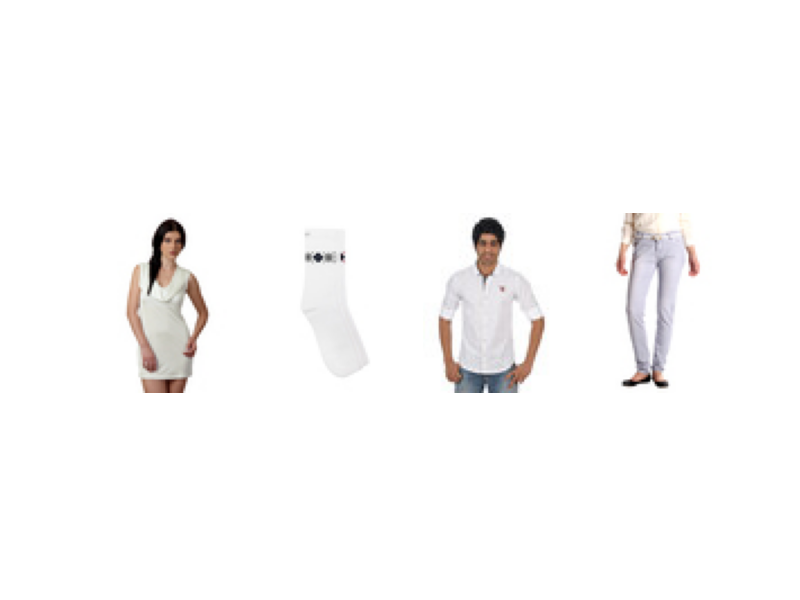
\includegraphics[width=.7\linewidth]{blancos_buenos.png}
  \caption*{50 primers White}
\end{minipage}%
\begin{minipage}{.5\textwidth}
  \centering
  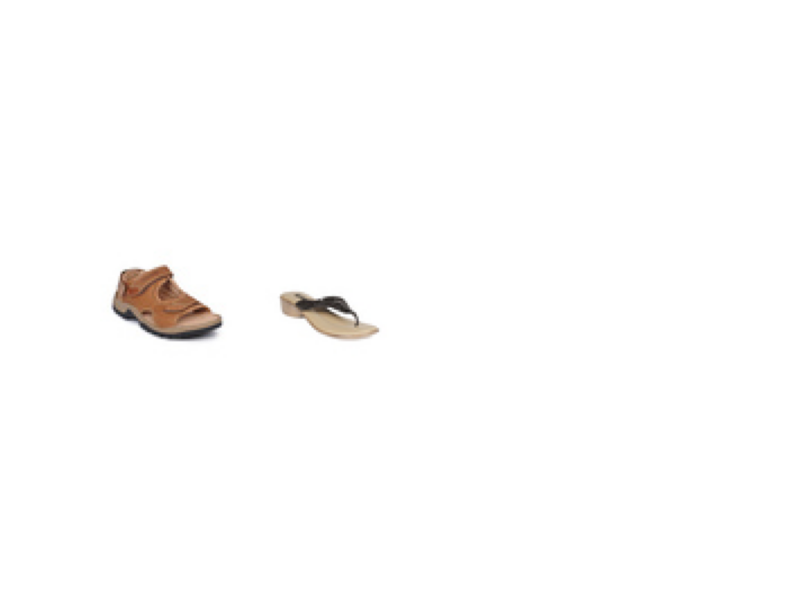
\includegraphics[width=.7\linewidth]{naranjito_bueno.png}
  \caption*{50 primers Orange}
\end{minipage}
\end{figure}

\newpage
\subsection{Retrieval\_by\_shape}\label{shape}
\subsubsection{Cdoc}
\begin{itemize}
    \item Entrada: 
    \begin{itemize}
        \item[$\circ$] Llista de les formes de cada imatge: \textbf{\textcolor{Turquoise}{knn\_shape}}
        \item[$\circ$] Llista de percentatges de formes a cada imatge: \textbf{\textcolor{Turquoise}{percentatge\_shape}}
        \item[$\circ$] Imatges etiquetades: \textbf{\textcolor{Turquoise}{imag}}
        \item[$\circ$] Llista de string que conté la forma que es vol buscar: \textbf{\textcolor{Turquoise}{question}}
    \end{itemize}
    \item Sortida: Conjunt d'imatges que contenen la forma desitjada i el seu percentatge.
    \item Funcionament: \\
    Per a cada imatge es comprova si té la forma desitjada, en cas afirmatiu es guarda l'índex de la imatge i el percentatge que representa la forma dins la imatge. Un cop mirades totes les imatges, la llista d'índexs s'ordena de menor a major segons el percentatge mencionat anteriorment. Finalment, es mostraran les imatges usant la funció \textcolor{funcblue}{visualize\_retrieval()} de la llibreria \textcolor{LimeGreen}{utils}.
\end{itemize}
Gràcies a les primeres execucions del programa vam veure que hi havia imatges molt mal etiquetades, ja que a vegades en una imatge apareixien dues peces de roba (p.e. una imatge de mitja cintura cap aball l'etiquetava com a samarreta, pantalons i sabates si també apareixien a la imatge).\\
\begin{figure}[h]
 \centering
    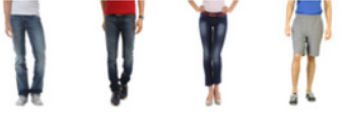
\includegraphics[width=0.55\textwidth]{shape_pocho.PNG}
\end{figure}\\
Aquesta mancança en el programa ens va fer aplicar les millores mencionades als primers apartats en aquesta funció per tal de millorar l'\texttt{accuracy}.\\
Un cop fetes les millores vam veure un augment considerable en la precisió dels resultats al demanar una forma concreta.

\newpage


\subsection{Retrieval\_combined}\label{combined}
\subsubsection{Cdoc}
\begin{itemize}
    \item Entrada: 
    \begin{itemize}
        \item[$\circ$] Llista de les formes de cada imatge: \textbf{\textcolor{Turquoise}{knn\_shape}}
        \item[$\circ$] Llista dels colors de cada imatge: \textbf{\textcolor{Turquoise}{kmeans\_color}}
        \item[$\circ$] Llista de percentatges de colors a cada imatge: \textbf{\textcolor{Turquoise}{percentatge\_color}}
        \item[$\circ$] Imatges etiquetades: \textbf{\textcolor{Turquoise}{imag}}
        \item[$\circ$] Llista de string que conté la forma que es vol buscar: \textbf{\textcolor{Turquoise}{question\_shape}}
        \item[$\circ$] Llista de string que conté els colors que es volen buscar: \textbf{\textcolor{Turquoise}{question\_color}}
    \end{itemize}
    \item Sortida: Mostra per pantalla les imatges de la forma demanada que contenen els colors demanats, usant la funció \textcolor{funcblue}{visualize\_retrieval()} de la llibreria \textcolor{LimeGreen}{utils}.
    \item Funcionament: \\
    Aquesta funció fa primer un KNN per filtrar segons la forma, seguidament d'un Kmeans per filtrar els colors.\\
    Per cada imatge que té la forma demanada, s'afegeix a una llista, i s'en creen dues, una amb el percentatge de colors i una altre amb els colors que conté, i es passen a la funció \textcolor{funcblue}{retrieval\_by\_color()}.
\end{itemize}
Com s'ha mencionat, aquesta funció és la unió de les dues anteriors, les combina per mostrar per pantalla el que demanem. Altre cop executant el programa sense cap millora implementada vam veure que s'havien de fer canvis. \\
Aquesta funció en ser una barreja de les dues anteriors, aplicant millores en aquestes dues va ser suficient per millorar aquesta tercera.

\begin{figure}[h]
 \centering
    \includegraphics[width=0.55\textwidth]{combined_chidoç.PNG}
\end{figure}\\

\newpage

\section{Kmeans}
\subsection{Introducció al Kmeans}
El Kmeans és un algorisme que permet trobar agrupacions de punts en una mostra, permentent així dividir i classificar la mostra en K classes diferents, cadascuna amb el centre d'inèrcia corresponent.\\\\
En el nostre classificador, el Kmeans és l'algorisme encarregat d'etiquetar les imatges pels colors que contenen, tenint en compte els percentatges de cada color.\\\\
Les millores implementades a l'algorisme han sigut prèviament explicades a l'apartat \textcolor{blue}{\ref{millores_implementades}}.
\newpage
\subsection{Get\_color\_accuracy}\label{matriucolors}
La finalitat d'aquesta funció consisteix en calcular que tan bo és l'etiquetatge del kmeans.
\subsubsection{CDoc}
\begin{itemize}
    \item Entrada: 
    \begin{itemize}
        \item[$\circ$] Colors de cada imatge: \textbf{\textcolor{Turquoise}{kmeans\_colors}}
        \item[$\circ$] Ground Truth dels colors de cada imatge: \textbf{\textcolor{Turquoise}{true\_label}}
    \end{itemize}
    \item Sortida: Llista que conté en ordre les accuracy \textit{intuicio}, \textit{tots correctes}, \textit{un correcte}, \textit{penalització} i \textit{colors correctes}.
    \item Funcionament: 
    \begin{enumerate}
        \item Intuició: Retorna la precisió de l'etiquetatge del kmeans segons la taula adjuntada a continuació, que dona a cada combinació etiqueta donada / etiqueta correcta un valor en quarts, de $0$ a $1$, representant l'acceptació que un color s'etiqueti d'una certa manera.
        
        \begin{figure}[h]
         \centering
            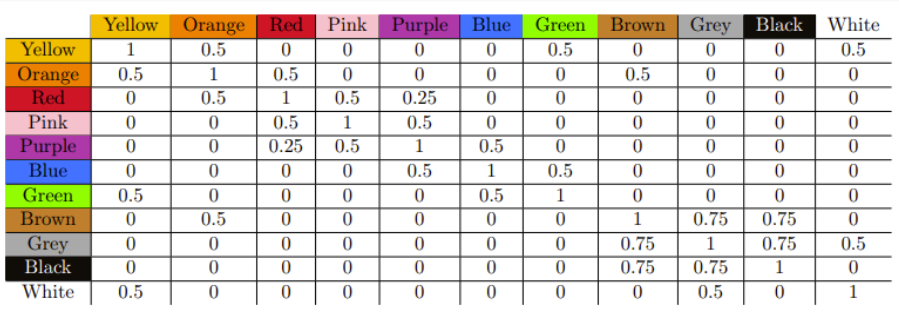
\includegraphics[width=0.55\textwidth]{matriu_colors.PNG}
        \end{figure}

        Per tal de confirmar el correcte funcionament de la taula, es va crear el següent mapa de calor, inspirat en una Confusion Matrix, que a l'eix horitzontal conté les etiquetes reals de cada imatge, i a l'eix vertical l'etiqueta que retorna el classificador, de manera que els colors més foscos representen una probabilitat més alta de ser etiquetats d'una certa manera, i els colors més suaus una probabilitat més baixa. 
        
         \begin{figure}[h]
         \centering
            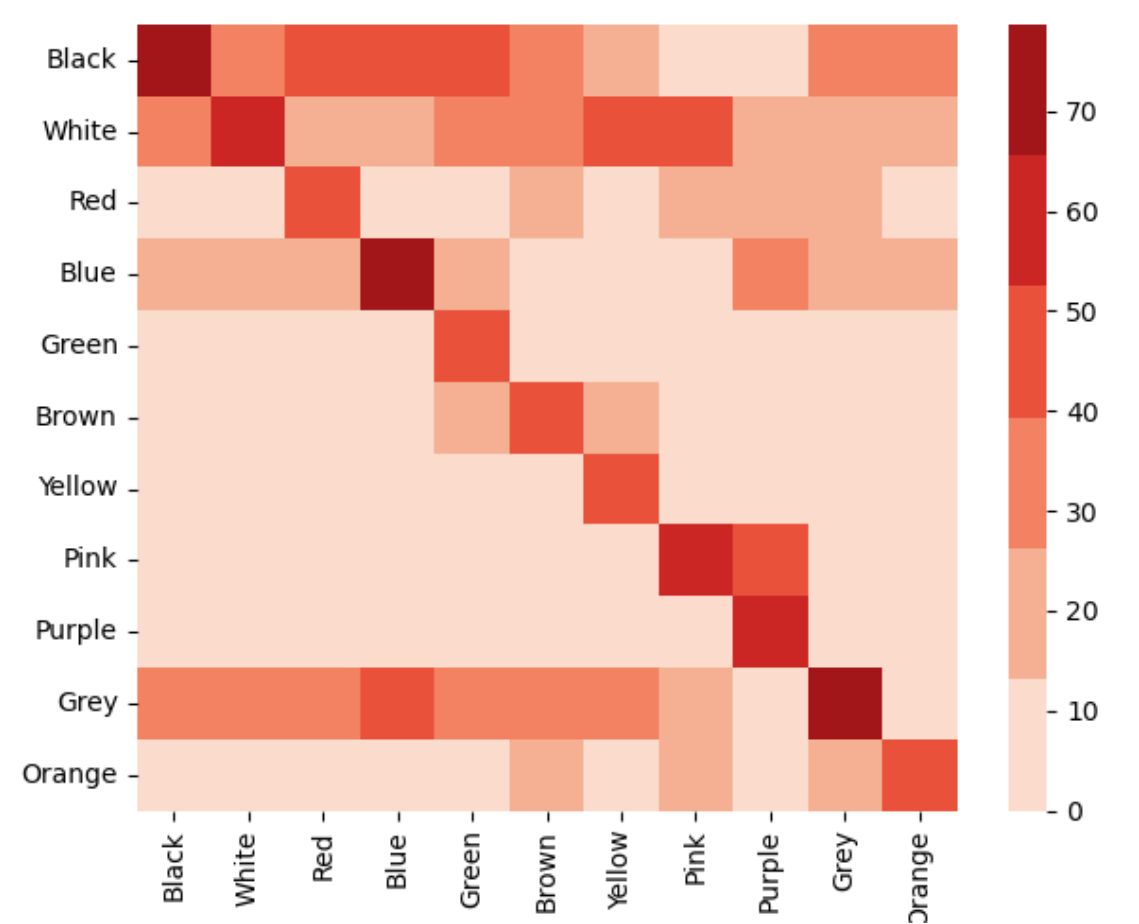
\includegraphics[width=0.35\textwidth]{mapa_calor.PNG}
        \end{figure}
        \item Tots correctes: Retorna la probabilitat que tots els colors que dona el classificador estiguin continguts a la llista $true\_colors$.
        \item Un correcte: Retorna la probabilitat que almenys un dels colors que dona el classificador estigui contingut a la llista $true\_colors$.
        \item Penalització: Retorna proporció $\frac{\text{Colors\_etiquetats } \cap \text{ Colors\_true\_label}}{\text{Colors\_etiquetats } \cup \text{ Colors\_true\_label}}$
        \item Colors correctes: Retorna el percentatge de quantes vegades s'ha etiquetat el mateix nombre de colors, tot i no ser aquests els mateixos.
    \end{enumerate}
\end{itemize}\\
Si s'executa la funció amb el Kmeans per defecte s'obté el següent resultat:
\begin{figure}[h]
    \centering
    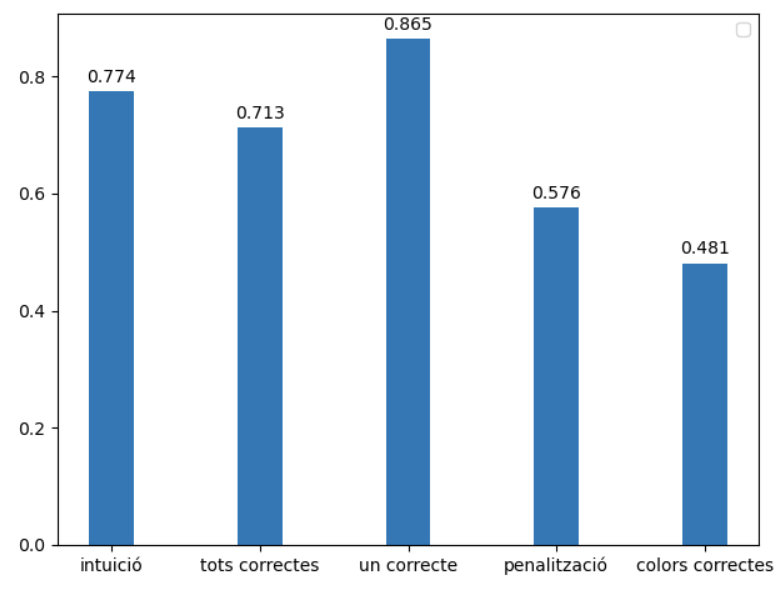
\includegraphics[width=.7\linewidth]{color_accuracy.PNG}
    \caption{precisions get\_color\_accuracy()}
    \label{fig:my_label}
\end{figure}
S'observa com hi han discrepacies en el mètode de calcular la precisió dels resultats. Per tal d'unificar els resultats en els analisis de les dades posterios s'ha decidit utilitzar el criterio de \textit{intuició} per a comparar l'accuracy de diversos mètodes i implementacions.

\newpage


\subsection{K\_statistics}

Aquesta funció veu l’eficiència en iteracions i temps segons la K triada del kmeans, això ho compara amb gràfiques generades (concretament nosaltres observant-les veiem quina K és millor).
\subsubsection{CDoc}

\begin{itemize}
     \item Entrada: 
    \begin{itemize}
        \item[$\circ$] K màxima a evaluar: \textbf{\textcolor{Turquoise}{k\_max}}
        \item[$\circ$] Les imatges etiquetades: \textbf{\textcolor{Turquoise}{imags}}
         \item[$\circ$] Diccionari de les opcions del Kmeans:
         \textbf{\textcolor{Turquoise}{options}}
    \end{itemize}
    \item Sortida: Mostra per pantalla tres gràfiques.\\
Una gràfica lineal de temps, un boxplot d'iteracions i un gràfic de barres.
    \item Funcionament: 
    Usa les opcions del kmeans introduïdes al diccionari $options$ per generar les gràfiques corresponents. Les diverses opcions a escollir són:
    
    \begin{itemize}
        \item[$\circ$] Inicialització dels centroides: \textit{KM\_INIT}.
        \item[$\circ$] Mètode per calcular la millor K: \textit{FITTING}.
        \item[$\circ$] Mètode per calcular una cota inferior per K: \textit{SELECTION}.
    \end{itemize}
    
\end{itemize}
A continuació s'exposen els diversos mètodes que s'han implementat al kmeans, i, per tant, els diversos mètodes que es poden usar per generar les gràfiques.\\\\
\underline{KM\_INIT}:
\begin{table}[h]
    \centering
    \begin{tabular}{ l | l }
        \textbf{Mètode} & \textbf{Explicació} \\ \hline\hline
        \textit{first} & Genera K centroides agafant els K primers píxels de la imatge \\ \hdashline
        \textit{random} & Genera K centroides agafant K píxels de la imatge de forma aleatòria \\ \hdashline
        \textit{colors} & S'usen els primers K colors diferents trobats a la imatge per generar els centroides \\ \hdashline
        \multirow{3}{*}{\textit{distance}} & S'agafa un píxel de la imatge de forma aleatòria, i els següents més allunyats dels \\
        & que tenim fins al moment; si K = 3, el tercer píxel seria el més allunyat del prime\\
        & r i segon alhora
    \end{tabular}
    \caption{Opcions del mètode KM\_INIT}
    \label{tab:my_label}
\end{table}\\
\underline{FITTING}:
\begin{itemize}
    \item Within Class Distance (\textit{WCD}): ha de ser baixa perquè el clúster sigui compacte. Usa la següent fòrmula:
    $$WCD = \sum_{i=1}^{k}  D(C_{j}), \text{ on } D(C) = \frac{2}{m(m-1)} \sum_{j=1}^{m}\sum_{i=j+1}^{m} d(x^i,x^j) : x^i, x^j \in C, i, j: 1...m$$
    \item Inter Class Distance (\textit{ICD}): ha de ser elevada perquè els clústers estiguin ben diferenciats. Usa la següent fòrmula:\\
$\begin{array}{ccc}
    \hspace{-1em} ICD = \sum_{j=1}^{k} \sum_ {i=j+1}^k D(C_{j},C_{i}), \text{ on } D(C_1, C_2) = \frac{1}{m_1m_2} \sum_{j=1}^{m_1}\sum_{i=1}^{m_2} d(x^i,x^j)
\end{array}\Bigg\{ \begin{array}{cc}
    x^i\in C_1:i:1...m_1 \\
    x^j \in C_2:j:1...m_2
\end{array}$
    \item Fisher Distance (\textit{FD}); ha de ser baixa perquè el clúster sigui compacte. Usa la fòrmula: 
    $$FD = \frac{WCD}{ICD}$$
\end{itemize}\\
\underline{SELECTION}:
\begin{table}[h]
    \centering
    \begin{tabular}{ l | l }
        \textbf{Mètode} & \textbf{Explicació} \\\hline\hline
        Default & Inicicialitza la K com $K=2$\\\hdashline
         \multirow{2}{*}{Canvas} & Agafa 1 de cada 50 píxels de la imatge, classifica els colors i el nombre \\
        & de colors diferents seran els K clústers inicials. \\\hdashline
        \multirow{2}{*}{Random} & Agafa el $10\%$ dels píxels de la imatge de forma aleatòria, classifica els \\
        & colors i els colors diferents seran els K clústers inicials.
    \end{tabular}
    \caption{Opcions per trobar cota inferior de K}
    \label{tab:my_label}
\end{table}

\newpage
\hspace{-1.5em}Els següents gràfics són un exemple d'$output$ usant les opcions KM\_INIT = first, FITTING = WCD i SELECTION = random.
\begin{figure}[h!]
\begin{minipage}{.3\textwidth}
  \centering
  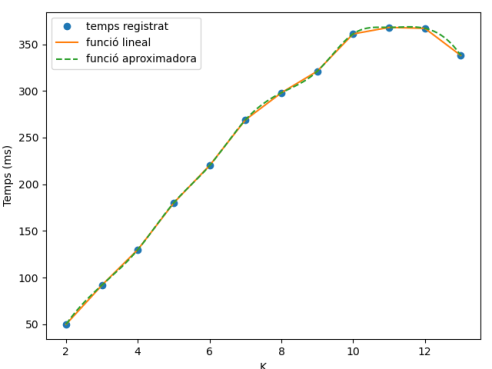
\includegraphics[width=.9\linewidth]{def_temps.png}
\end{minipage}%
\begin{minipage}{.3\textwidth}
  \centering
  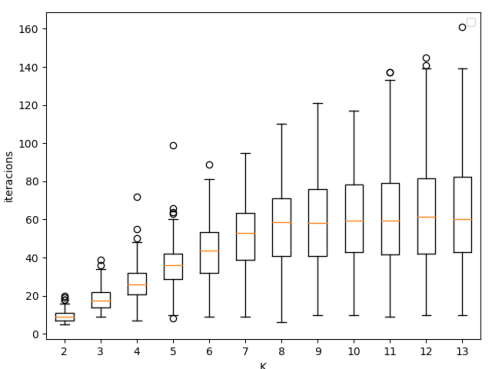
\includegraphics[width=.9\linewidth]{def_iter.png}
\end{minipage}
\begin{minipage}{.3\textwidth}
  \centering
  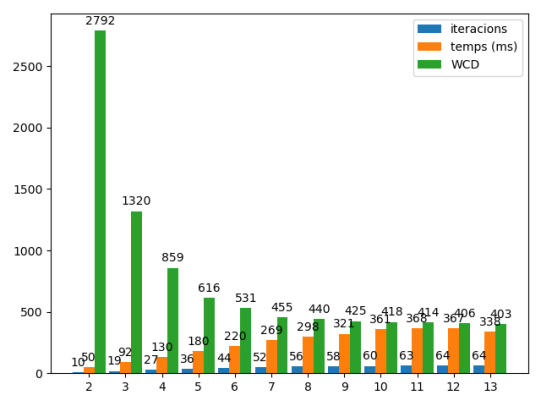
\includegraphics[width=.9\linewidth]{def_barras.png}
\end{minipage}
\end{figure}\\
Per altra banda, els següents gràfics s'han generat usant les opcions KM\_INIT = random, FITTING = WCD i SELECTION = random.
\label{fig:grafico}
\begin{figure}[h]
\begin{minipage}{.3\textwidth}
  \centering
  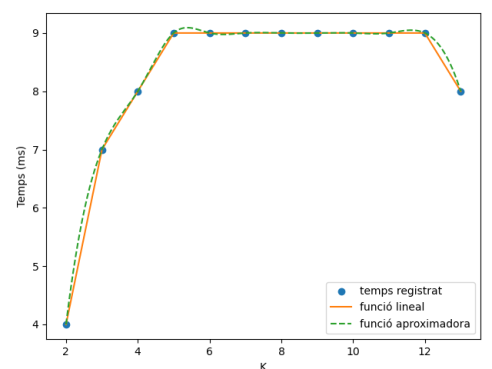
\includegraphics[width=.9\linewidth]{rnd_temps.png}
\end{minipage}%
\begin{minipage}{.3\textwidth}
  \centering
  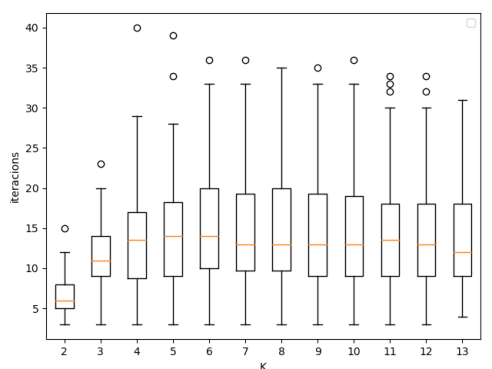
\includegraphics[width=.9\linewidth]{rnd_iter.png}
\end{minipage}
\begin{minipage}{.3\textwidth}
  \centering
  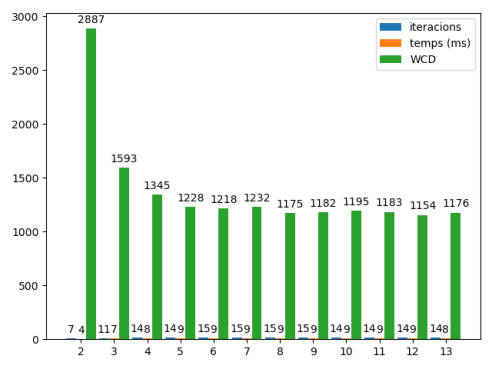
\includegraphics[width=.9\linewidth]{rnd_barras.png}
\end{minipage}
\end{figure}



\newpage

\subsubsection{Anàlisi dels resultats per heurístiques}
Per tal de trobar la K a utilitzar per classificar un dataset, s'han estudiat les iteracions i temps que triga el Kmeans per valors de K entre 2 i 13 (inclosos), usant les 3 heurístiques implementades; WCD (Within Class Distance), ICD (Inter Class Distance) i la FD (Fisher Distance). Els gràfics obtinguts han sigut els següents:
\begin{figure}[h!]
\centering
\begin{minipage}{.33\textwidth}
  \centering
  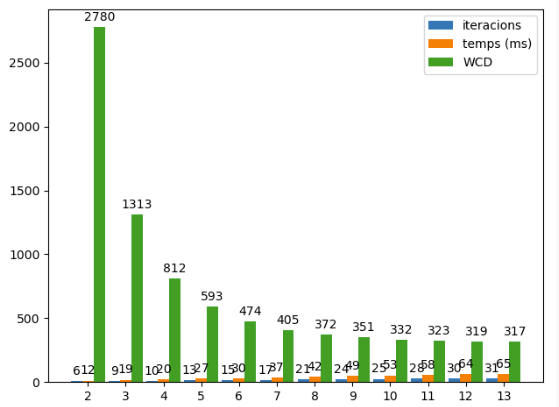
\includegraphics[width=.8\linewidth]{kstatisticsWCD.PNG}
\end{minipage}%
\begin{minipage}{.33\textwidth}
  \centering
  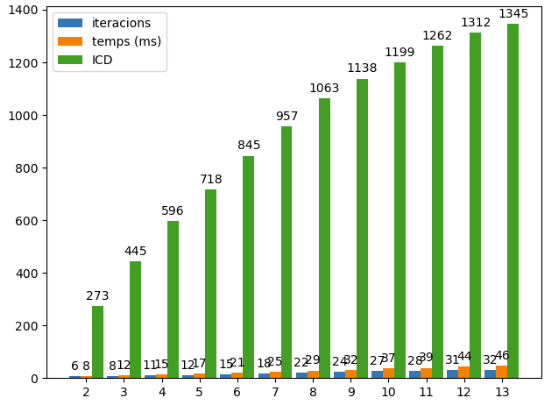
\includegraphics[width=.8\linewidth]{kstatisticsICD.PNG}
\end{minipage}%
\begin{minipage}{.33\textwidth}
  \centering
  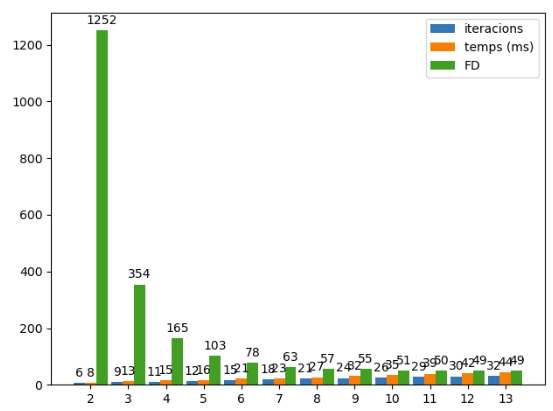
\includegraphics[width=.8\linewidth]{kstatisticsFD.PNG}
\end{minipage}
\end{figure}
\justify
S'observa com la distància intra-class i el discriminant de fisher ràpidament disminueixen, i pel contrari, la distància intra-class augmenta, de la manera que cal esperar. Observem que la millor K es situa al voltant de 3 i 8 de manera intuitiva i també veiem com la distancia de fisher decideix d'una manera més eficient el valor de K ja que interrelaciona els dos paràmetres més important a l'hora d'agrupar els clústers (la distància inter i intra class).
\newpage

\subsubsection{Anàlisi dels resultats per inicialització dels centroides}
S'han estudiat el nombre d'iteracions i el temps que triga el KMeans per a cada K començant per a K=2 fins a K=13, menys pel mètode \textit{colors}, on la K màxima és 11. Es fa l'estudi amb l'objectiu de veure si les propostes noves d'inicialització, \textit{colors} i \textit{distance}, suposen una millora respecte a les ja implementades.
\center\underline{First:}
\begin{figure}[h!]
\centering
\begin{minipage}{.5\textwidth}
  \centering
  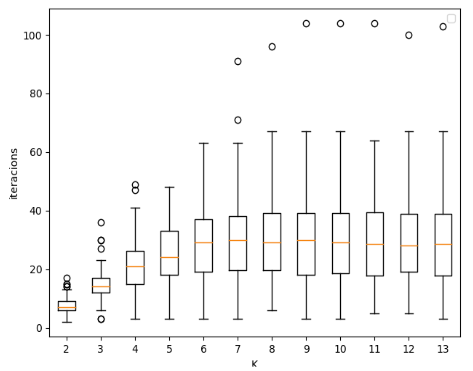
\includegraphics[width=.8\linewidth]{boxplot_default_centroides.PNG}
\end{minipage}%
\begin{minipage}{.5\textwidth}
  \centering
  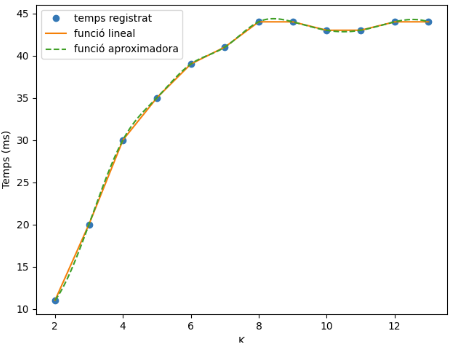
\includegraphics[width=.8\linewidth]{temps_default_centroides.PNG}
\end{minipage}
\end{figure}
\justify
S'observa com ràpidament la mediana del nombre d'iteracions s'estabilitza al voltant de les 30 iteracions, i no es veuen masses outliers, és més es pot deduïr que el que apareix per a K altes és la mateixa imatge. Pel que respecte als quartils, es veu que no són massa petits, i per tant el nombre d'iteracions és bastant diferent per a cada imatge, i per tant l'eficiència depent molt de com és la imatge.\\
Respecte al temps, és veu un creixement lineal fins a K=9, on s'estabilitza al voltant dels 45 milisegons. És en general, bastant lent.
\newpage
\center\underline{Random:}
\begin{figure}[h!]
\centering
\begin{minipage}{.5\textwidth}
  \centering
  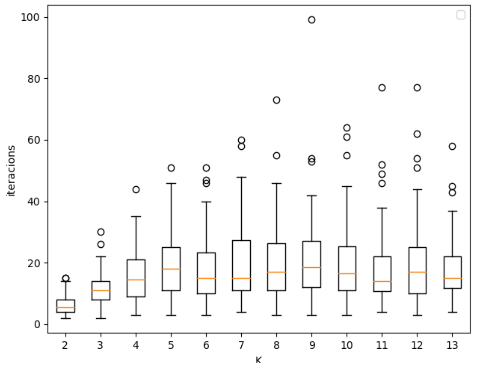
\includegraphics[width=.8\linewidth]{boxplot_random_centroides.PNG}
\end{minipage}%
\begin{minipage}{.5\textwidth}
  \centering
  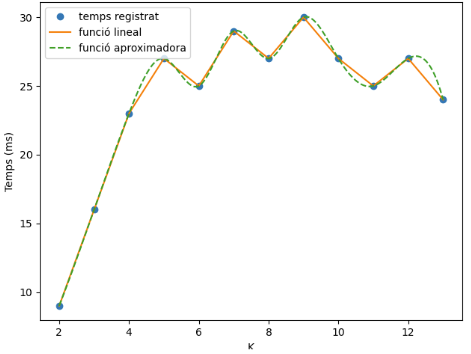
\includegraphics[width=.8\linewidth]{temps_random_centroides.PNG}
\end{minipage}
\end{figure}
\justify
S'observa com la mediana del nombre d'iteracions s'estabilitza una mica per sota de les 20 iteracions, i no es veuen masses outliers, és més es pot deduïr que el que apareix per a K altes és la mateixa imatge. Pel que respecte als quartils, es veu que no són massa grans, i per tant el nombre d'iteracions es pot deduïr que és bastant semblant independentment de la imatge.\\
Respecte al temps, creix linealment fins a K=5, i a partir d'allà té pics depenent de si es tracta d'una K parella o una senar, tot i que la diferència en temps no és massa gran. Això succeix a l'interval de temps de 25 milisegons i 30, per tant independentment de si és K parella o senar, el temps és bastant bo. 


\center\underline{Colors:}
\begin{figure}[h!]
\centering
\begin{minipage}{.5\textwidth}
  \centering
  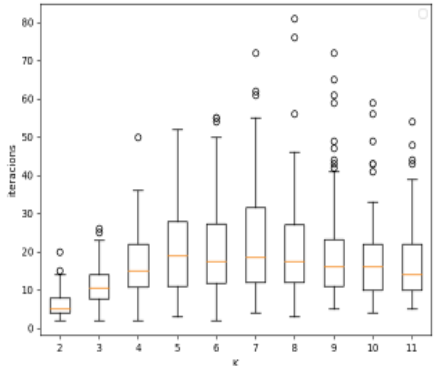
\includegraphics[width=.8\linewidth]{boxplot_colors_centroides.PNG}
\end{minipage}%
\begin{minipage}{.5\textwidth}
  \centering
  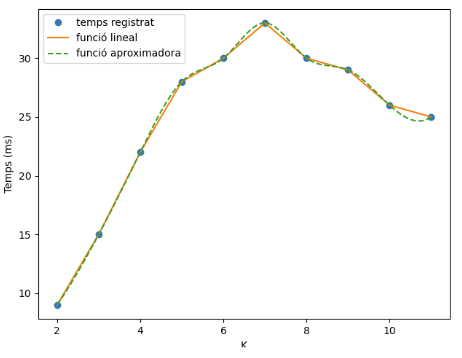
\includegraphics[width=.8\linewidth]{temps_color_centroides.PNG}
\end{minipage}
\end{figure}
\justify
S'observa com la mediana del nombre d'iteracions s'estabilitza entre 10 i 20 iteracions, i no es veuen masses outliers amb excepció de per K=9, on es pot deduïr que aquestes excepcions es deuen a imatges amb pocs colors on cap dels colors està entre els 9 seleccionats. Pel que respecte als quartils, semblan bastant grans, tot i que es pot veure fàcilment a que les iteracions depenen exclusivament de quins colors s'han seleccionat, i de si aquests es troben a la imatge o no, i per tant al ser completament aleatori és normal que el nombre d'iteracions no sigui massa uniforme .\\
Respecte al temps, creix linealment fins a K=7, i a partir d'allà decreix linealment, ja que al haver-hi més colors inicials com a centroides, és més senzill fer els clústers dels colors que apareixen a la imatge. El pic de temps és d'uns 35 milisegons, el qual es considera ja bastant alt, però per K altes com 10 i 11 (màxim per a aquest mètode) triga al voltant de 25 milisegons, el qual és un bon temps.
\center\underline{Distance:}
\begin{figure}[h!]
\centering
\begin{minipage}{.5\textwidth}
  \centering
  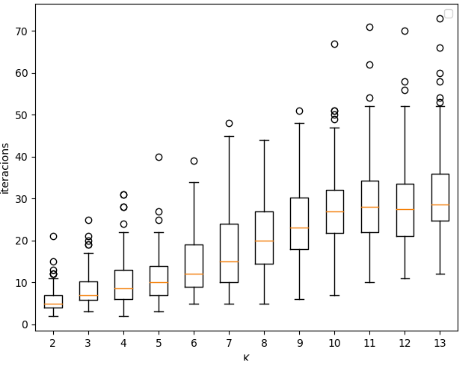
\includegraphics[width=.8\linewidth]{boxplot_distance_centroides.PNG}
\end{minipage}%
\begin{minipage}{.5\textwidth}
  \centering
  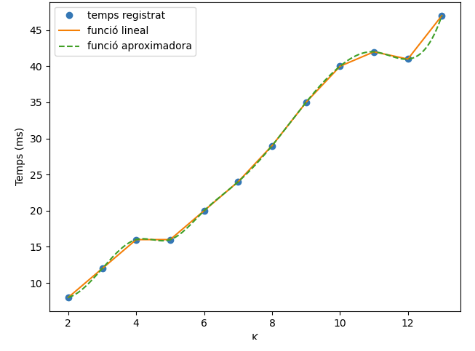
\includegraphics[width=.8\linewidth]{temps_distance_centroides.PNG}
\end{minipage}
\end{figure}
\justify
S'observa com el nombre d'iteracions va augmentant a mesura que creix K, i no sembla estabilitzar-se en cap moment. No es veuen masses outliers tampoc.
Pel que respecte als quartils, no semblen massa grans, i per tant el nombre d'iteracions no sembla dependre de la imatge.
Al fixar-se en la funció de temps, aquest creix quasi linealment amb K, ja que un major nombre de centroides implica un major nombre de càlculs de distàncies. Aquest fet fa que per K altes el temps sigui bastant dolent, mentre que és el primer mètode que no passa dels 25 milisegons abans de K=8.
\\\\
Vist tots els mètodes, el més evident és que First és el pitjor de tots. Guiant-nos pel nombre d'iteracions i el temps per a totes les K, sembla ser que els dos millors mètodes són \textit{random} i \textit{colors}, sent lleugerament millor el mètode \textit{random} en ambdos apartats.
Això ens podria fer pensar que és el millor mètode a utilitzar per a l'etiquetatge, però com s'ha pogut observar a l'apartat d'anàlisi d'heurístiques, la gran majoria d'imatges convergeixen abans de K=8 (els valors més freqüents mirant la gràfica de la Fisher Distance semblan ser 4,5 i 6). Per tant el millor mètode per a aquest programa en concret és aquell que tingui el menor nombre d'iteracions i el menor temps en K $\leq 8$, i aquest mètode resulta que és el distance. És lògic que ho sigui, ja que l'algorisme fa que els centroides inicials estiguin ja ben separats i que siguin de colors que apareixen a la imatge sempre, que porta a un nombre menor d'iteracions, i al ser una K petita el cost dels càlculs de les distàncies no és massa gran, i té més rellevancia en el temps el nombre d'iteracions.

\newpage

\subsection{Lower\_bound}
Per optimitzar l'eficiència amb la que trobar la millor K, va sorgir la idea de trobar una cota inferior per a aquesta, i així tenir una K inicial respectiva a la imatge que s'esta processant. S'han proposat tres mètodes per a determinar aquesta cota inferior.\\\\
El primer d'ells, anomenat default, no correspon a cap modificació del codi. S'inicia per una K preestablerta, que en aquest cas s'ha decidit que sigui 2, al considerar que sempre una mica del color del background (al no ser factible treure'l tot amb els mètodes implementats) i el color de la peça de roba, que segur és diferent al fons.\\\\
També s'ha fet la implementació del mètode canvas, on s'agafen punts ja predeterminats del canvas, és a dir com si es fes una graella. En concret, un cop tret el background de la imatge, agafa píxels equiespaiats a 50 píxels de distància, i els guarda a una llista. Llavors aprofitant la funció \textcolor{funcblue}{get\_colors()} veure a quin color correspon cada píxel, i decidir la K inicial a partir dels colors únics trobats.\\\\
Com a última implementació s'ha fet el mètode random, que segueix una filosofia semblant al canvas, però en comptes d'escollir píxels equiespaiats, agafa una petita quantitat aleatòriament de la imatge ja sense background. Aleshores segueix el mateix procediment que canvas per a decidir la K inicial.\\
Analitzem ara les diferències en temps d'execució:\\

\newpage

\subsubsection{Anàlisi del lower-bound}
Amb els diferents mètodes implementats cal veure el rendiment del KMeans, on els paràmetres interessants a estudiar per a aquesta funció són el temps mitjà que triga l'algorisme en donar etiquetes per a cada imatge i per a quina K comença. Per a poder realitzar aquest anàlisi s'ha fet una gràfica lineal on l'eix de les abscisses representa el temps i el de les ordenades la K. El resultat és la gràfica següent:
\begin{figure}[h!]
\centering
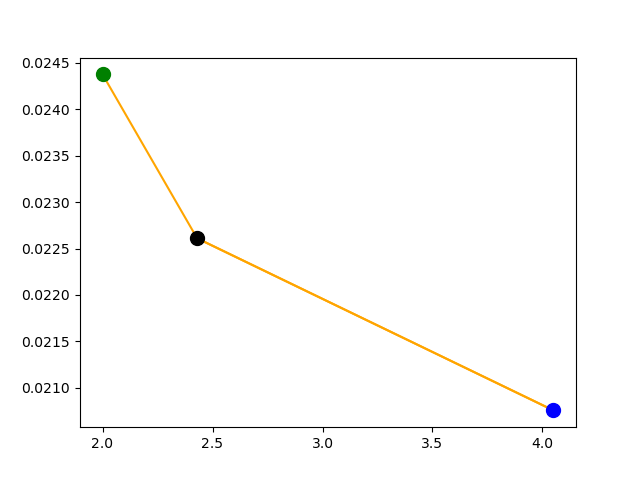
\includegraphics[scale=0.6]{lower.png}
\caption*{\footnotesize Verd = Default | Negre = Canvas | Blau = Random}
\end{figure}\\
Es pot observar fàcilment com els dos mètodes per a trobar un lower bound d'acord amb la imatge són bastant millors al que ja estava implementat, el default, que sempre comença per K=2 i és el que té un temps mig més alt.\\
Pel que fa als mètodes de canvas i random, el que ens porta a la major eficiència és el de random, degut a que la seva K mitjana inicial, aproximadament 4, és major a la de canvas. Si la K per la que s'acostumès a parar l'algorisme (és a dir el nombre de colors finals donats) fos 2 o 3, és a dir, valors de K més propers a la K mitja obtinguda pel mètode canvas, segurament aquest mètode fos millor que random. No obstant això, s'ha vist en l'anàlisi de les heurístiques que les K per les quals l'agoritme acostuma a parar són 4 i 5, i per tant començar per una K major, con és el cas de random, resulta més eficient.\\
En conclusió, la implementació d'una cota inferior millora l'eficiència de l'algoritme, i en concret aconseguir aquesta cota mirant els colors del píxels seleccionats de manera aleatòria és la millor opció.

\newpage


\subsection{Best\_k\_statistics}\label{bestkstatistics}
S'encarrega d'evaluar amb cada heurística com evoluciona el temps d'execució, la K i el valor de l'heurística segons el percentatge preestablert a partir del qual es decideix no seguir, que va avançant segons el paràmetre $factor$.
\subsubsection{CDoc}
\begin{itemize}
    \item Entrada: 
    \begin{itemize}
        \item[$\circ$] Imatges a evaluar: \textbf{\textcolor{Turquoise}{imags}}
        \item[$\circ$] Factor amb el que avança el percentatge: \textbf{\textcolor{Turquoise}{fact}}
    \end{itemize}
    \item Sortida: Retorna 9 gràfics que mostren l'evolució del temps, heurística i valor de la K usant diferents percentatges entre 0 i 1, amb les 3 heurístiques implementades: WCD, ICD i FD.
    \item Funcionament: 
    Realitza un \textit{Kmeans} per cada heurística: WCD, ICD i FD, guardant a les llistes corresponents els valors de temps, heurística i K segons el llindar utilitzar, generant els gràfics.\\
    A continuació es mostra un exemple d'output de la funció:
    \begin{figure}[h!]
    \centering
    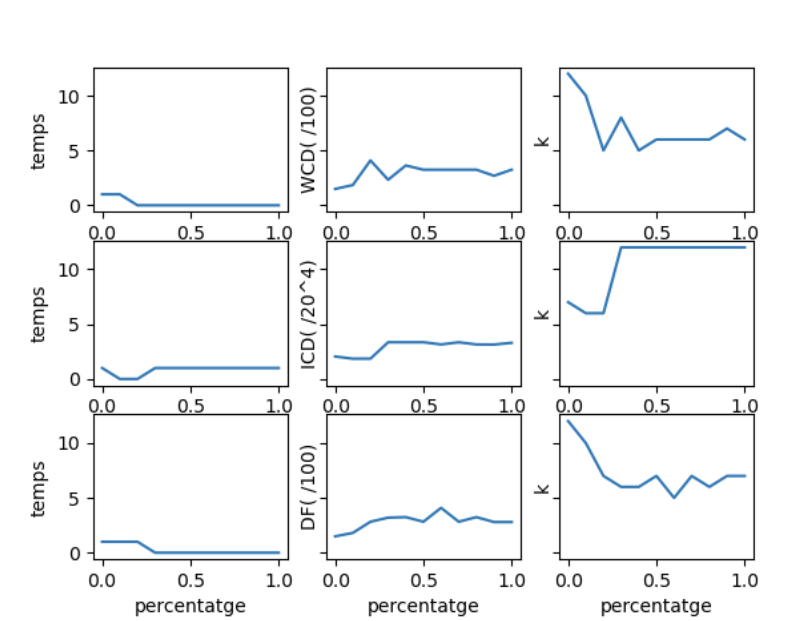
\includegraphics[scale=0.6]{best_k_statistics_percentatges.PNG}
    \end{figure}
\end{itemize}
\newpage
\subsection{Anàlisis sobre la informació redundant}
Un dels objectius que s'han marcat era estudiar quanta informació era rellevant per tal de fer una bona classificació.\\
Partint de la suposició de que els colors es distribueixen amb la mateixa proporció agafant una mostra aleatòria que agafant el conjunt total de la imatge, es pot classificar tota la imatge només usant aquest subconjunt.\\
Es corfirma la hipòtesis estudiant el comportament del classificador comparant els resultats obtinguts amb un subconjunt aleatori del $10\%$ de la imatge i la totalitat d'ella. Mostrem ara els resultats obtinguts.
\begin{figure}[h!]
\centering
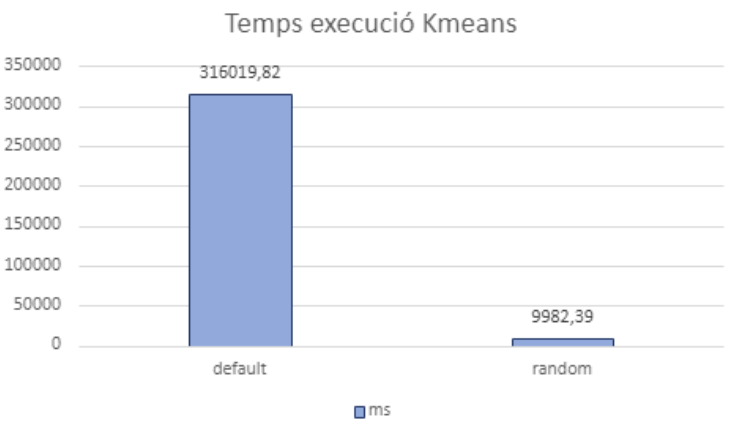
\includegraphics[scale=0.6]{temps_execucio_kmeans.PNG}
\end{figure}
S'observa doncs una millora significativa del temps d'execució, concretament, del $3100\%$. Aquestes dades han sigut obtingudes amb la mitja de temps d'execució amb tot el dataset del que es disposa.\\
L'anàlisi sobre la precisió es fa a l'apartat \textcolor{blue}{\ref{fig:grafico}}.\\
Es conclou que no cal tenir en compte tota la informació per classificar, amb una subpart ja classifica degudament.
\newpage

\subsection{Analisis de la precisió de les diferents implementacions}
Es recull una taula amb el temps d'execució i la precisió obtinguda per les diferents implementacions:
\begin{table}[h]
    \centering
    \begin{tabular}{ l | l | l }
        \textbf{Implementació} & \textbf{Temps} & \textbf{Accuracy} \\\hline\hline
        kmeans default all data (first, WCD, no lower bound) & $0.08124613761901$ & $0.7956944444444$ \\ \hdashline
        kmeans default 0.1 data (first, WCD, no lower bound) & $0.03273582458496$ & $0.7729044261652$ \\ \hdashline
        kmeans 0.1 data (random, WCD, lowerbound-canvas) & $0.03170824050901$ & $0.7678858206032$ \\ \hdashline
        kmeans 0.1 data (random, WCD, lowerbound-random) & $0.03176188468933$ & $0.7810810810810$ \\ \hdashline
        kmeans 0.1 data (colors, WCD, lowerbound-random) & $0.04948639869689$ & $0.7869761065410$ \\ \hdashline
        kmeans 0.1 data (distance, WCD, lowerbound-random) & $0.03317117691040$ & $0.7977036819428$ \\ \hdashline 
        kmeans 0.1 data (distance, ICD, lowerbound-random) & $0.04856395721435$ & $0.7954612220916$ \\ \hdashline 
        kmeans 0.1 data (distance, FD, lowerbound-random) & $0.05337095260620$ & $0.7931502154321$ \\ \hdashline 
        Kmeans 0.1 data (distance, WCD, no lower bound) & $0.03028964996337$ & $0.7825744222483$ 
    \end{tabular}
    \caption{Analisis de les implementacions del kmeans més rellevants}
    \label{tab:resultats_kmeans}
\end{table}\\
Dels resultats s'observa com kmeans que obté la millor accuracy és \textit{kmeans 0.1 data (distance, WCD, lowerbound-random)} i el que obté el resultat de manera més ràpida és \textit{Kmeans 0.1 data (distance, WCD, no lower bound)}. 

\newpage

\section{KNN}
\subsection{Introducció al KNN}
El KNN és un algorisme que estima el representant de cada classe, i assigna a la resta de punts la classe del veí més proper.\\\\
En el nostre classificador, el KNN és l'algorisme encarregat d'etiquetar les imatges per les formes que contenen, donant una o dues etiquetes a cada imatge depenent dels percentatges de les formes contingudes en cada una.\\\\
Les millores implementades a l'algorisme han sigur prèviament explicades a l'apartat \textcolor{blue}{\ref{millores_implementades}}.
\newpage

\subsection{Get\_shape\_accuracy}
La finalitat d'aquesta funció consisteix en calcular que tan bo és l'etiquetatge del kmeans.
\subsubsection{CDoc}
\begin{itemize}
    \item Entrada: 
    \begin{itemize}
        \item[$\circ$] Llista de tuples de les etiquetes de la forma de cada imatge: \textbf{\textcolor{Turquoise}{kmeans\_shape}}
        \item[$\circ$] Ground Truth dels colors de cada imatge: \textbf{\textcolor{Turquoise}{true\_label}}
    \end{itemize}
    \item Sortida: Llista que conté en ordre les accuracy: \textit{ primera etiqueta correcta}, \textit{segona etiqueta correcta}, \textit{alguna de les dues correcta}.
    \item Funcionament: 
    Es creen dues llistes que s'omplen amb la primera i la segona etiqueta de la imatge respectivament. En cas que la imatge només tingui una etiqueta, al lloc de la segona a la llista s'hi insereix un espai en blanc.

    D'aquestes llistes es marquen amb un 0 les etiquetes incorrectes i amb un 1 les correctes.
    \begin{enumerate}
        \item Primera etiqueta correcta: Retorna el quocient $\frac{etiquetes\_1\_correctes}{len(true\_labels)}$
        \item Segona etiqueta correcta: Retorna el quocient $\frac{etiquetes\_2\_correctes}{len(true\_labels)}$
        \item Alguna correcta: Retorna el quocient $\frac{etiquetes\_1\_2\_correctes}{len(true\_labels)}$
        
    \end{enumerate}
\end{itemize}
\newpage
\subsection{Implementacions del KNN}
Per tal de trobar la manera més òptima de classificar per formes, s'ha decidit programar 2 mètodes (a part del default) per veure com evolucionava l'eficiència de l'etiquetador.\\
Expliquem ara aquestes implementacions.\\
\subsubsection{Mètode \textit{Grey}}
Una de les implementacions era classificar cada imatge de la manera "estàndard" \hspace{0.250em}però reduint la quantitat d'informació que obteniem per imatge, intentant quedar-nos només amb la més rellevant.\\
El procés decidit per aquesta reducció en la informació que es té ha sigut passar la imatge a escala de grisos. La resta dels càlculs és equivalent al KNN per \textit{default}.\\

\subsubsection{Mètode \textit{Area}}
Una de les implementacions era classificar cada imatge segons un únic valor, de manera que només calgués comparar-les mirant quant s'assembla aquest valor.\\
S'ha decidit d'entre totes les opcions que el valor que se li otorga a cada imatge és la proporció entre el nombre de píxels de la figura i el nombre de píxels del fons.\\
Aquesta proporció, semblant al quocient de les àrees que ocupa el fons i la figura en la imatge, és el que denominem com mètode \textit{area}.\\
\newpage
\subsection{Anàlisi de les implementacions}
Per tal d'analitzar l'eficiència de les diverses implementacions, s'ha utilitzat la funció abans explicada \textcolor{funcblue}{get\_shape\_accuracy()}.\\
Els resultats obtinguts han sigut els següents:
\begin{figure}[h]
 \centering
  \subfloat[Mètode \textit{default}]{
    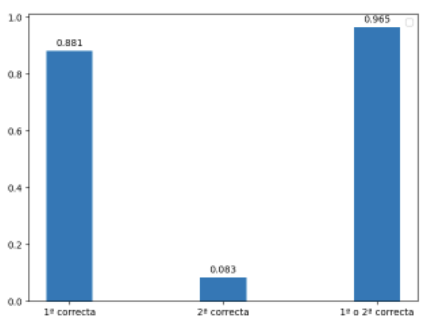
\includegraphics[width=0.3\textwidth]{shape_accuracy_default.PNG}}
  \subfloat[Mètode \textit{grey}]{
    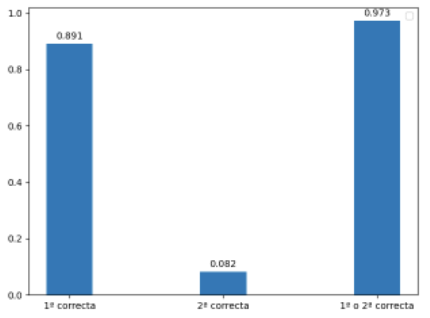
\includegraphics[width=0.3\textwidth]{get_shape_accuracy_grey.PNG}}
  \subfloat[Mètode \textit{area}]{
    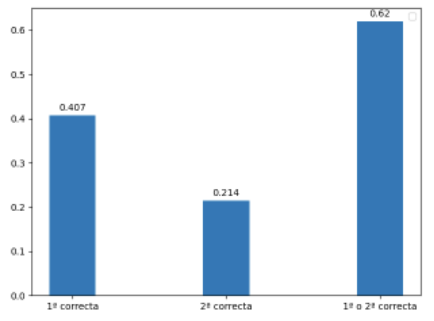
\includegraphics[width=0.3\textwidth]{get_shape_accuracy_area.PNG}}
\end{figure}\\
Dels gràfics obtinguts es poden observar diverses coses:
\begin{enumerate}
    \item El mètode amb millor accuracy és el grey.
    \item No hi ha molta diferència en l'accuracy entre el default i el grey.
    \item El mètode area té una eficiència qüestionable, ja que recau molta part de la seva precisió en la segona etiquetació.
\end{enumerate}
Es continua l'anàlisis dels resultats analitzant el temps d'execució de cada un dels mètodes.\\
\begin{figure}[h]
  \begin{center}
    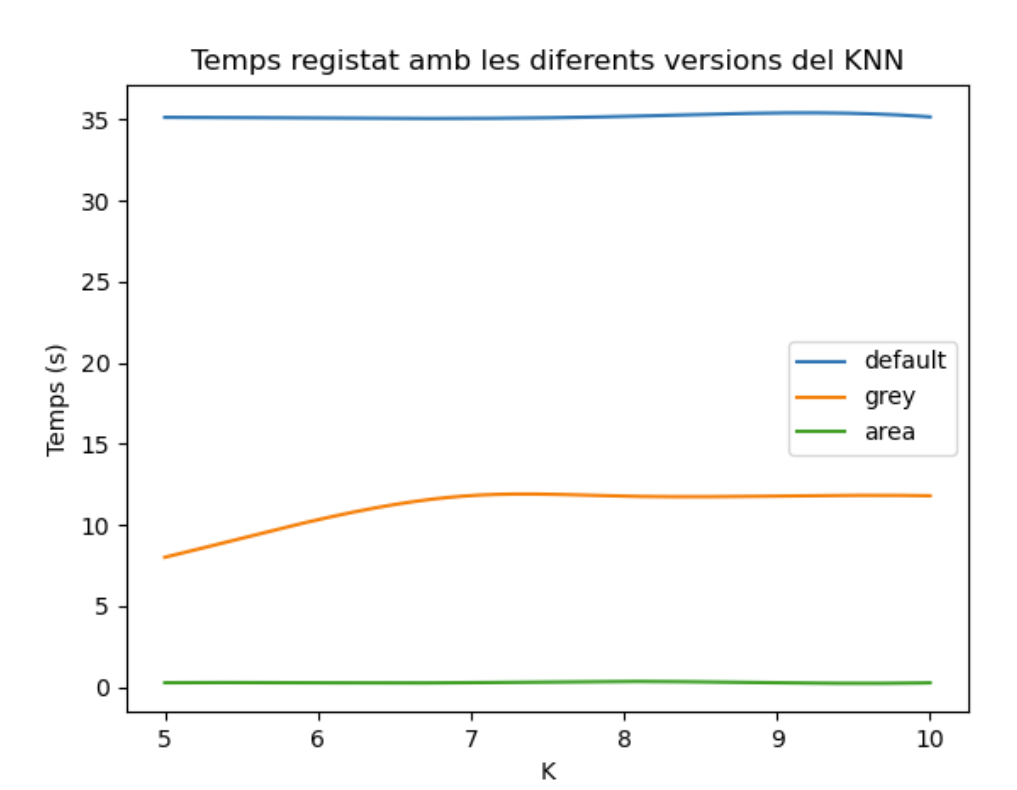
\includegraphics[width=0.6\textwidth]{comparacio_temps_knn.PNG}
  \end{center}
\end{figure}
S’observa a l’eix d’ordenades el temps que es triga en classificar tot el dataset de test i en l’eix d’absisses la K.\\
Cal destacar la gran millora en el temps del KNN segons el mètode de l’àrea ja que sembla que per a qualsevol K sigui constant. Per la poca quantitat de dataset que disposem aquesta millora de temps és irrelevant degut a la poca precisió, tot i que si el dataset fos molt gran, podria ser una opció a tenir en compte. \\
Doncs, es conclou que el mètode que té millor relació temps/accuracy és el grey, que s’estabilitza a partir de K=7.


\newpage
\subsection{CrossValidation}\label{crossvalidation}
Es va decidir trobar la millor K mitjançant un Cross Validation.\\
Degut a que no podem utilitzar el test dataset per validar el valor de la K, s'ha utilitzat una subpart aleatòria del train dataset. Per a cada KNN inicialitzat amb la funció \textcolor{funcblue}{KFolds\_CrossValidationsKNN()}, es fa el predict (usant la funció \textcolor{funcblue}{predict\_cross\_validation()}) amb el bloc de dades no utilitzat per a fer validació. Ho fa per 4 subdatasets, comprova l’accuracy dels 4 i fa la mitja dels accuracy obtinguts. Això ho fa a partir de mirar K veïns. \\\\
Arrel de no poder usar el test dataset, no es pot assegurar que les dades obtingudes siguin suficientment precisses, pel que es dona un interval de confiança del 95\% que està contingut entre les línies discontinues vermella i verda de la imatge adjuntada a continuació:

\begin{figure}[h!]
\centering
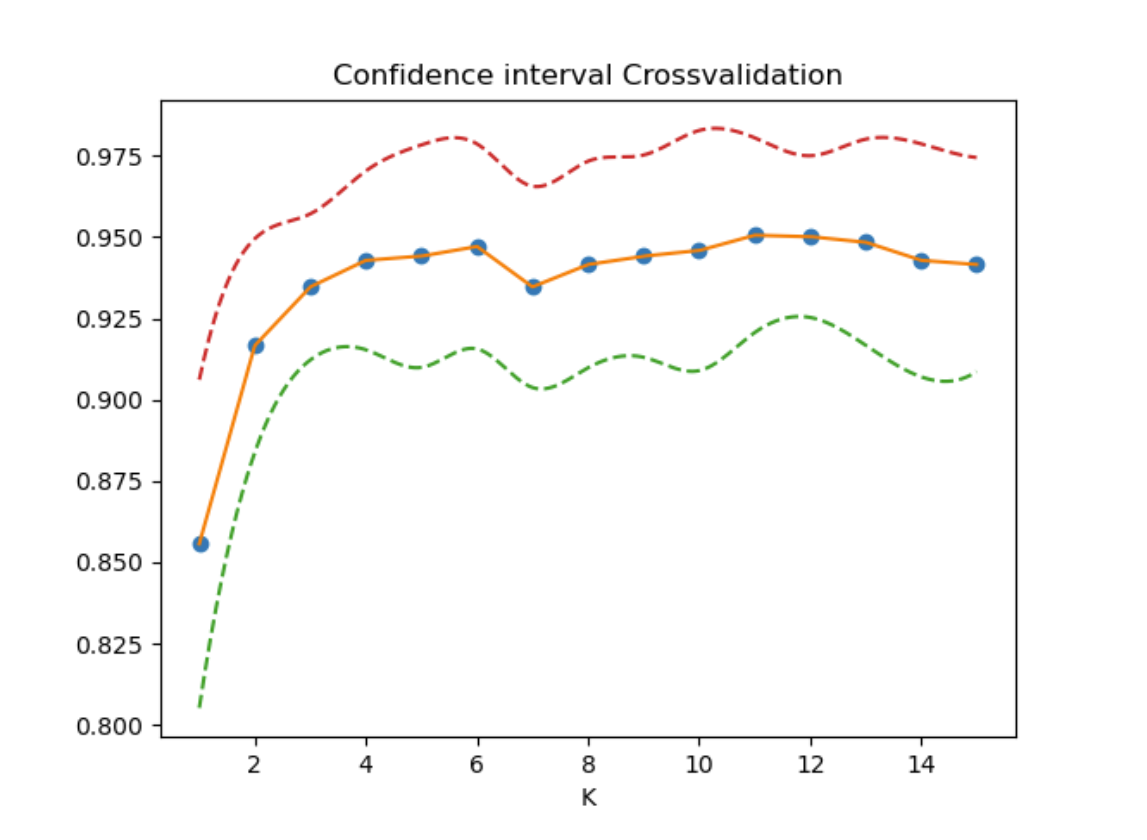
\includegraphics[scale=0.5]{crossvalidation.PNG}
\end{figure}
\hspace{-1.5em}Al gràfic s'observa el percentatge d’acerts (\textit{accuracy}) obtinguts per diferents valors de K entre $1$ i $15$. A més, s’ha interpolat de manera lineal entre ells per veure la tendència, que s'estabilitza a partir de $K=3$ amb una precisió d'entre el 90\% i el 98\%. Es dedueix així, que la K que proporciona millor accuracy és la 11 ja que té el límit inferior de l'interval de confiança més elevat.\\\\
Com s'ha mencionat anteriorment, degut a l’alt cost computacional d'aquest apartat del classificador, s'ha vist necessari implementar un multiprocessing, que ha permès baixar molt significativament el temps de còmput del programa.
\newpage

\section{Conclusions}

\subsection{Kmeans}
Després de realitzar les millores pertinents al k-means i fer el seu anàlisis corresponent, hem arribat a unes certes conclusion. Aquestes són les següents:
\begin{enumerate}
    \item La primera i la més important és la millora significativa del temps d'execució en seleccionar només un $10\%$ de la imatge de manera aleatòria, ja que s'ha demostrat amb els anàlisis pertinents que decreix en un $3100\%$ i, a més, la presició augmenta.
    \item De tots els mètodes implementats, el que dona una millor accuracy és el kmeans que usa la inicialització de centroïdes \textit{distance}, la heurística WCD, i que usa una cota inferior per la $K$ trobada amb el mètode \textit{random}. Aquest mètode té una precisió del $79.8\%$ i un temps d'execució de $0.033$ segons.
    \item Dels mètodes implementats, el més lent és el kmeans que inicialitza els centroïdes amb la opció \textit{first}, usa la heurística \textit{WCD} i no usa una cota inferior per la $K$, tot i que dona una precisió molt alta (del $79.6\%$) i un temps de $0.08$ segons.
    \item Finalment el mètode més ràpid de tots és el kmeans on els centroïdes s'inicialitzen segons la \textit{distance}, s'usa d'heurística \textit{WCD} i no usa cap cota inferior per la $K$. Té un temps de $0.030$ segons i una precisió del $78\%$.
\end{enumerate}
\newpage

\subsection{KNN}
Després de realitzar les millores pertinents al knn i fer el seu anàlisis corresponent,  hem arribat a unes certes conclusion. Aquestes són les següents:
\begin{enumerate}
    \item Encara que el mètode \textit{àrea} té poca precisió, un $62\%$ i, per tant, amb el nostre dataset no és útil fer-lo servir, això és degut a la poca quantitat d'imatges que es volen etiquetar, i en cas de tenir un dataset molt gran a classificar, seria una opció a tenir en compte, ja que redueix molt el temps d'execució (triga entre $0$ i $1$ segon a classificar tot el dataset de test), que sembla ser constant per qualssevol valor de $K$.
    \item La millor $K$ pel dataset donat és la $6$.
    \item Els mètodes que usen $K=6$ donen una millor precisió que la resta.
    \item Si no tinguéssim el \textit{ground truth}, la millor $K$ seria la $11$, ja que s'ha provat amb el \textit{Cross Validation} que és la que s'assegura de donar millor precisió, ja que té el límit inferior més elevat de l'interval de confiança.
    \item De les diverses combinacions que s'han implementat pel KNN, la que dona una millor relació temps/accuracy és el grey.
    \item La implementació del \textit{multiprocessing} a certes parts del programa ha sigut acertada ja que ha disminuït molt significativament el temps de còmput.
\end{enumerate}


\end{document}
